%%%%%%%%%%%%%%%%%%%%%%%%%%%%%%%%%%%%%%%%%
% Short Sectioned Assignment
% LaTeX Template
% Version 1.0 (5/5/12)
%
% This template has been downloaded from:
% http://www.LaTeXTemplates.com
%
% Original author:

% Frits Wenneker (http://www.howtotex.com)
%
% License:
% CC BY-NC-SA 3.0 (http://creativecommons.org/licenses/by-nc-sa/3.0/)
%
%%%%%%%%%%%%%%%%%%%%%%%%%%%%%%%%%%%%%%%%%

%----------------------------------------------------------------------------------------
%	PACKAGES AND OTHER DOCUMENT CONFIGURATIONS
%----------------------------------------------------------------------------------------

\documentclass[paper=a4, fontsize=11pt]{scrartcl} % A4 paper and 11pt font size

\usepackage[T1]{fontenc} % Use 8-bit encoding that has 256 glyphs
\usepackage{fourier} % Use the Adobe Utopia font for the document - comment this line to return to the LaTeX default
\usepackage[english]{babel} % English language/hyphenation
\usepackage{amsmath,amsfonts,amsthm} % Math packages

\usepackage{lipsum} % Used for inserting dummy 'Lorem ipsum' text into the template

\usepackage{enumitem}
\usepackage{mathtools}
\DeclarePairedDelimiter\ceil{\lceil}{\rceil}
\DeclarePairedDelimiter\floor{\lfloor}{\rfloor}
\usepackage{graphicx}
\usepackage{subfig}	
\usepackage{listings}
\usepackage{amsmath}
\usepackage{algorithm}
\usepackage[noend]{algpseudocode}
\makeatletter
\def\BState{\State\hskip-\ALG@thistlm}
\makeatother

\usepackage{sectsty} % Allows customizing section commands
\allsectionsfont{\centering \normalfont\scshape} % Make all sections centered, the default font and small caps

\usepackage{fancyhdr} % Custom headers and footers
\pagestyle{fancyplain} % Makes all pages in the document conform to the custom headers and footers
\fancyhead{} % No page header - if you want one, create it in the same way as the footers below
\fancyfoot[L]{} % Empty left footer
\fancyfoot[C]{} % Empty center footer
\fancyfoot[R]{\thepage} % Page numbering for right footer
\renewcommand{\headrulewidth}{0pt} % Remove header underlines
\renewcommand{\footrulewidth}{0pt} % Remove footer underlines
\newcommand{\itab}[1]{\hspace{0em}\rlap{#1}}
\newcommand{\tab}[1]{\hspace{.2\textwidth}\rlap{#1}}

\setlength{\headheight}{13.6pt} % Customize the height of the header

\numberwithin{equation}{section} % Number equations within sections (i.e. 1.1, 1.2, 2.1, 2.2 instead of 1, 2, 3, 4)
\numberwithin{figure}{section} % Number figures within sections (i.e. 1.1, 1.2, 2.1, 2.2 instead of 1, 2, 3, 4)
\numberwithin{table}{section} % Number tables within sections (i.e. 1.1, 1.2, 2.1, 2.2 instead of 1, 2, 3, 4)

\setlength\parindent{0pt} % Removes all indentation from paragraphs - comment this line for an assignment with lots of text

%----------------------------------------------------------------------------------------
%	TITLE SECTION
%----------------------------------------------------------------------------------------

\newcommand{\horrule}[1]{\rule{\linewidth}{#1}} % Create horizontal rule command with 1 argument of height
\title{	
\normalfont \normalsize 
\textsc{University of Toronto, Department of ECE} \\ [25pt] % Your university, school and/or department name(s)
\horrule{0.5pt} \\[0.4cm] % Thin top horizontal rule
\huge ECE1762 - Homework 4 \\ % The assignment title
\horrule{2pt} \\[0.5cm] % Thick bottom horizontal rule
}

\author{Xinyun Lv(1001091178), Yang Wang(1001319227)} % Your name

\date{\normalsize\today} % Today's date or a custom date

\begin{document}

\maketitle % Print the title
\section{Problem I}
\textbf{solution}:\\
Let $G'$ be the DAG on the strongly connected components of $G$. Number the nodes of $G^{'}$ in some topological order. We claim that $G$ is semiconnected iff there is always a path from the $i$-th node to the $j$-th node of $G'$ if $i < j$.  

\begin{figure}[h]
	\centering
	\subfloat[Subfigure 1 list of figures text][$G$ is semiconnected]{
		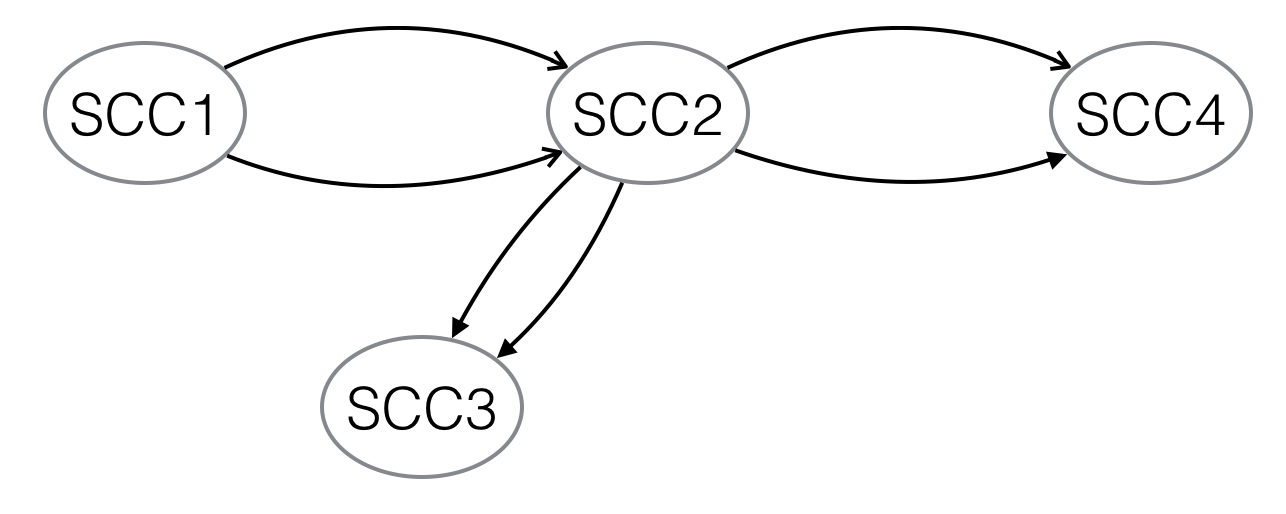
\includegraphics[width=0.4\textwidth]{hw4p1b}
		\label{fg:p1a}}
	\subfloat[Subfigure 2 list of figures text][$G$ is not semiconnected]{
		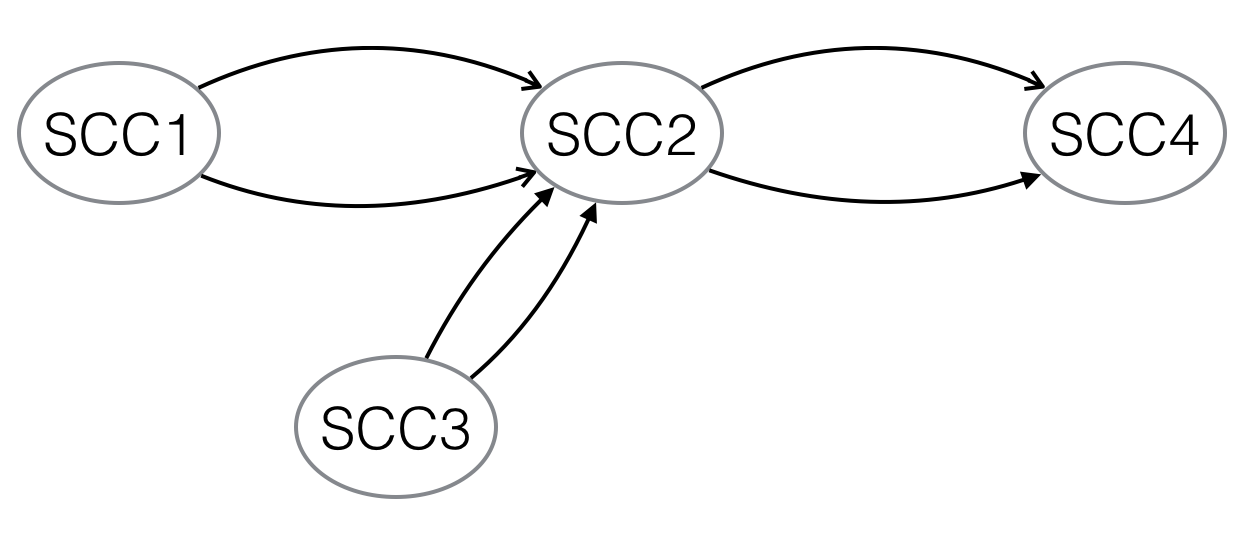
\includegraphics[width=0.4\textwidth]{hw4p1a}
		\label{fg:p1b}}
	\caption{Examples}
	\label{fg:p1}
\end{figure}

Suppose that there is always a path from the $i$-th node to the $j$-th node of $G'$ if $i < j$. Then, for any two vertices $u$ and $v$ in $G$, they either belong to the same SCC (in which case there is a path from $u$ to $v$ and a path from $v$ to $u$), or they belong to two different SCC's, $c_u$ and $c_v$. Without loss of generality, suppose $c_u$ occurs earlier than $c_v$ with respect to the topological order. Then, by hypothesis, there is a path from $c_u$ to $c_v$, so there is a path from $u$ to $v$ as desired. As shown in the Figure \ref{fg:p1a}.\\

Now suppose that for some topological sort of $G'$, there is no path from the $i$-th node (with respect to this sort) to the $j$-th node, where $i < j$. Then, there can be no path from the $j$-th node to the $i$-th node since $i < j$ and the nodes are topologically sorted. Hence, if $u$ is a vertex lying in the $i$-th SCC and $v$ a vertex lying in the $j$-th SCC, there are no paths from $u$ to $v$ or from $v$ to $u$, so $G$ is not semiconnected. As shown in the Figure \ref{fg:p1b}.\\

This observation allows us to devise an algorithm to determine if $G$ is semiconnected: we first compute the strongly connected components of $G$ and construct the graph $G'$ in time $O(\mid V \mid + \mid E \mid)$. Then, using DFS from any vertex in $G'$, we can topologically sort $G'$ in $O(\mid V \mid  + \mid E \mid)$ time. Now, we check if there is a path from the $i$-th SCC to the $j$-th SCC if $i < j$. Note that this is the case iff there is an edge in $G'$ from the $i$-th SCC to the $(i + 1)$-th SCC. Hence, we can just scan through the topological sort in $O(\mid V \mid)$ time to see if the $i$-th SCC has an edge to the $(i + 1)$-th SCC. The total running time of the algorithm is $O(\mid V \mid + \mid E \mid)$.
\section{Problem II}
\textbf{solution}:\\
To find a path from $s$ to $v$ that has minimum bottleneck-length among all paths from $s$ to $v$, we could use the idea of Dijkstra algorithm and change its relaxation function. We define $d[v], v \in V$ as the bottleneck-length of vertex $v$. If d[v] > max{d[u], w(u, v)}, $(u, v) \in E$, we update d[v] = max{d[u], w(u, v)}. We also define $\pi[v]$ as the parent node of each $v \in V$. At the end of the algorithm, we can get the minimum bottleneck-length among all paths from $s$ to $v$. The pseudo-code is as follows:\\

$d[s] \gets -\infty
$\\
$S \gets \Phi$\\
\textbf{for} each $v \in V - \left\{ s \right\}$:\\
 \hspace*{0.6cm} \textbf{do} $d[v] \gets \infty$\\
 $Q \gets V$\\
 \textbf{while} $Q \neq \Phi$\\
 \hspace*{0.6cm} $u \gets Extract\_min(Q)$\\
 \hspace*{0.6cm} \textbf{for} each $v \in adj[u]$:\\
 \hspace*{0.6cm} \hspace*{0.6cm} \textbf{do} if d[v] > max\{d[u], w(u, v)\}\\
\hspace*{0.6cm} \hspace*{0.6cm} \hspace*{0.6cm} d[v] $\gets$ max\{d[u], w(u, v)\}\\
\hspace*{0.6cm} \hspace*{0.6cm} \hspace*{0.6cm} $\pi[v] \gets u$\\

Similar with Dijkstra algorithm, we can achieve a running time of $O(VlogV + E)$ by implementing the min-priority queue with a Fibonacci heap. The amortized cost of each of the Extract-Min operations if $O(logV)$ and there are $\mid V \mid$ such operations. Meanwhile, each Decrease-Key call, of which there are at most $\mid E \mid$, takes only $O(1)$ amortized time. 
\section{Problem III}
\textbf{solution}:\\
Suppose $d_j$ is the first edge that violate $c_i \leq d_i$ which means $c_j > d_j$. Since $d_1 \leq d_2 \leq \dots \leq d_j$ then we have $d_1 \leq d_2 \leq \dots \leq d_j < c_j$. \\

There are two conditions at this point:
\begin{enumerate}
  \item $c_i = d_i$ for all $i < j$
  \item There is at least one pair of edge have $c_m \neq d_m$ 
\end{enumerate}

For the first condition, we have $c_i = d_i$ for all $i < j$. Because $c_j > d_j$, which implies that we once considered $d_j$ before $c_j$ but $d_j$ will form a cycle during Kruskal algorithm. However, since $c_i = d_i$ for all $i < j$, $d_j$ will also form a cycle in the arbitrary spanning tree $\Rightarrow$ a contradiction.\\

For the second condition, we assume that $c_m \neq d_m$, $m < j$ and $c_j > d_m$. This means that we have also once considered $d_m$ but $d_m$ will form a cycle during Kruskal algorithm so we choose $c_m$ instead. Which implies that $c_m > d_m$, so, $d_m$ is the first edge that violate $c_j \leq d_j$. But $d_j$ is the first edge that violate $c_i \leq d_i$ $\Rightarrow$ a contradiction. 

\section{Problem IV}
\textbf{solution}:\\
We could use the idea of Kruskal's algorithm. At the beginning of the algorithm we could treat each node $v \in V$ as a cluster so that we have $\mid V \mid$ cluster at beginning. The algorithm runs as follows:\\

$A \gets \Phi$\\
\textbf{for} each $v \in V[G]$\\
\hspace*{0.6cm} \textbf{do} Make-Set($v$)\\
sort the edges of $E$ into nondecreasing order by weigt $w$\\
$i \gets \mid V \mid - k$\\
\textbf{while} $i \geq 0$\\
\hspace*{0.6cm} edge $(u, v) \in E$, taken in nondecreasing order by weight\\
\hspace*{0.6cm} \textbf{do if} Find-Set(u) $\neq$ Find-Set(v)\\
\hspace*{0.6cm} \hspace*{0.6cm} \hspace*{0.6cm} \textbf{then} $A \gets A \cup \{(u, v)\}$\\
\hspace*{0.6cm} \hspace*{0.6cm} \hspace*{0.6cm} Union($u$, $v$)\\
\hspace*{0.6cm} $i \gets i - 1$\\

We start from the lightest edge, each time we take an edge in nondecreasing order by weight whose two endpoints belongs to different cluster. Thus, we merge two clusters each time. If we take this operation $\mid V \mid - k$ times, we will have $k$ clusters eventually. We now claim that after $\mid V \mid - k$ rounds, our algorithm guarantees that the minimum distance between any pairs in two different resulting clusters is maximized. We can prove it as follows:\\

When $k = 1$, the algorithm above is actually the Kruskal's algorithm which we will get a MST. We will use this MST in the following proof. We can delete the $k - 1$ most expensive edges from the MST. The spacing $d$ of the clustering $C$ that this produces is the length of the $(k - 1)^{st}$ most expensive edge. Let $C'$ be a different clustering. We'll show that $C'$ must have the same or smaller separation than $C$. Since $C \neq C'$, there must be some pair $p_i, p_j$ that are in the same cluster in $C$ but different clusters in $C'$. \\

Together in $C$ $\Rightarrow$ Path $P$ between $p_i, p_j$ with all edges $\leq d$. Some edge of $P$ passes between two different cluster of $C'$. Therefore, $d$ is the maximized minimum distance. \\

The running time of this algorithm is $O(ElogV)$.







\section{Problem V}
\textbf{solution}:\\
To prove sufficiency in the directed case, let $(G, u, s, t)$ be a network with unit capacities $u = 1$ such that $t$ is reachable rfrom $s$ even after deleting any $k - 1$ edges. This implies that the minimum capacity of an $s-t$ cut is at least $k$. By the Max-Flow-Min-Cut Theorem this flow can be decomposed into integral flows on $s-t$ paths. Since all capacities are 1 we must have at least $k$ edge-dijoint $s-t$ paths. \\

To prove sufficiency in the undirected case, let $G$ be an undirected graph with two vertives $s$ and $t$ such that $t$ is reachable from $s$ even after deleting any $k - 1$ edges. This property obiously remains true if we replace each undirected edge $e = \left\{ v, w \right\}$  by five directed edges $(v, x_e), (w, x_e), (x_e, y_e), (y_e, v), (y_e, w)$ where $x_e$ and $y_e$ are new vertives. Now we have a digraph $G'$ and, by the first part, $k$ edge-disjoint $s-t$ paths in $G'$. These can be easily transformed to $k$ edge-disjoint $s-t$ pahts in $G$. 
\section{Problem VI}
\begin{enumerate}[label=(\alph*)]
	\item \textbf{solution:}\\
	The capacity of a cut is defined to be the sum of the capacities of the edges crossing it. Since the number of such edges is at most $\mid E \mid$, and the capacity of each edge is at most $C$, the capacity of any cut of $G$ is at most $C\mid E \mid$.

	\item \textbf{solution:}\\
	The capacity of an augmenting path is the minimum capacity of any edge on the path, so we are looking for an augmenting path whose edges all have capacity at least $K$ . Do a breadth-first search or depth-first-search as usual to find the path, considering only edges with residual capacity at least $K$ . (Treat lower-capacity edges as though they don't exist.) This search takes $O(V + E) = O(E)$ time since in flow network we have $\mid V \mid = O(E)$

	\item \textbf{solution:}\\
	Max-Flow-By-Scaling uses the Ford-Fulkerson method. It repeatedly augments the flow along an augmenting path until there are no augmenting paths of capacity greater than 1. Since all the capacities are integers, and the capacity of an augmenting path is positive, this means that there are no augmenting paths in the residual graph at the end of the algorithm. Thus, by the max-flow min-cut theorem, Max-Flow-By-Scaling returns a maximum flow.

	\item \textbf{solution:}\\
	The first time line 4 is executed, the capacity of any edge in $G_f$ equals its capacity in $G$, and by part (a) the capacity of a minimum cut of $G$ is at most $C\mid E \mid$. Initially $K = 2\lfloor lgC \rfloor$, hence $2K = 2 \cdot 2^{\lfloor lgC \rfloor} = 2^{\lfloor lgC \rfloor + 1} > 2^{lgC} = C$. So the capacity of a minimum cut of $G_f$ is initially less than $2K \mid E \mid$.\\

	The other times line 4 is executed, $K$ has just been halved, so the capacity of a cut of $G_f$ is at most $2K \mid E \mid$ at line 4 if and only if that capacity was at most $K \mid E \mid$ when the while loop of lines 5-6 last terminated. So we want to show that when line 7 is reached, the capacity of a minimum cut of $G_f$ is most $K \mid E \mid$.\\

	Let $G_f$ be the residual network when line 7 is reached.\\
	There is no augmenting path of capacity $\geq K$ in $G_f$\\
	$\Rightarrow$ max flow $f'$ in $G_f$ has value $\mid f' \mid < K \mid E \mid$\\
	$\Rightarrow$ min cut in $G_f$ has capacity $< K \mid E \mid$ 

	\item \textbf{solution:}\\
	By part (d), when line 4 is reached, the capacity of a minimum cut of $G_f$ is at most $2K \mid E \mid$, and thus the maximum flow in $G_f$ is at most $2K \mid E \mid$.\\

	By an extension of Lemma 26.2, the value of the maximum flow in $G$ equals the value of the current flow in $G$ plus the value of the maximum flow in $G_f$ . Therefore, the maximum flow in $G$ is at most $2K \mid E \mid$ more than the current flow in $G$. Every time the inner while loop finds an augmenting path of capacity at least $K$ , the flow in $G$ increases by $\geq K$ . Since the flow cannot increase by more than $2K \mid E \mid$, the loop executes at most $(2K \mid E \mid)/K = 2 \mid E \mid$ times.

	\item \textbf{solution:}\\
	The time complexity is dominated by the loop of lines 4-7. The outer while loop executes $O(lgC)$ times, since $K$ is initially $O(C)$ and is halved on each iteration, until $K < 1$. By part (e), the inner while loop executes $O(E)$ times for each value of $K$; and by part (b), each iteration takes $O(E)$ time. Thus, the total time is $O(E^2 lg C)$.
\end{enumerate}
\end{document}